
\begin{figure}
  \centering 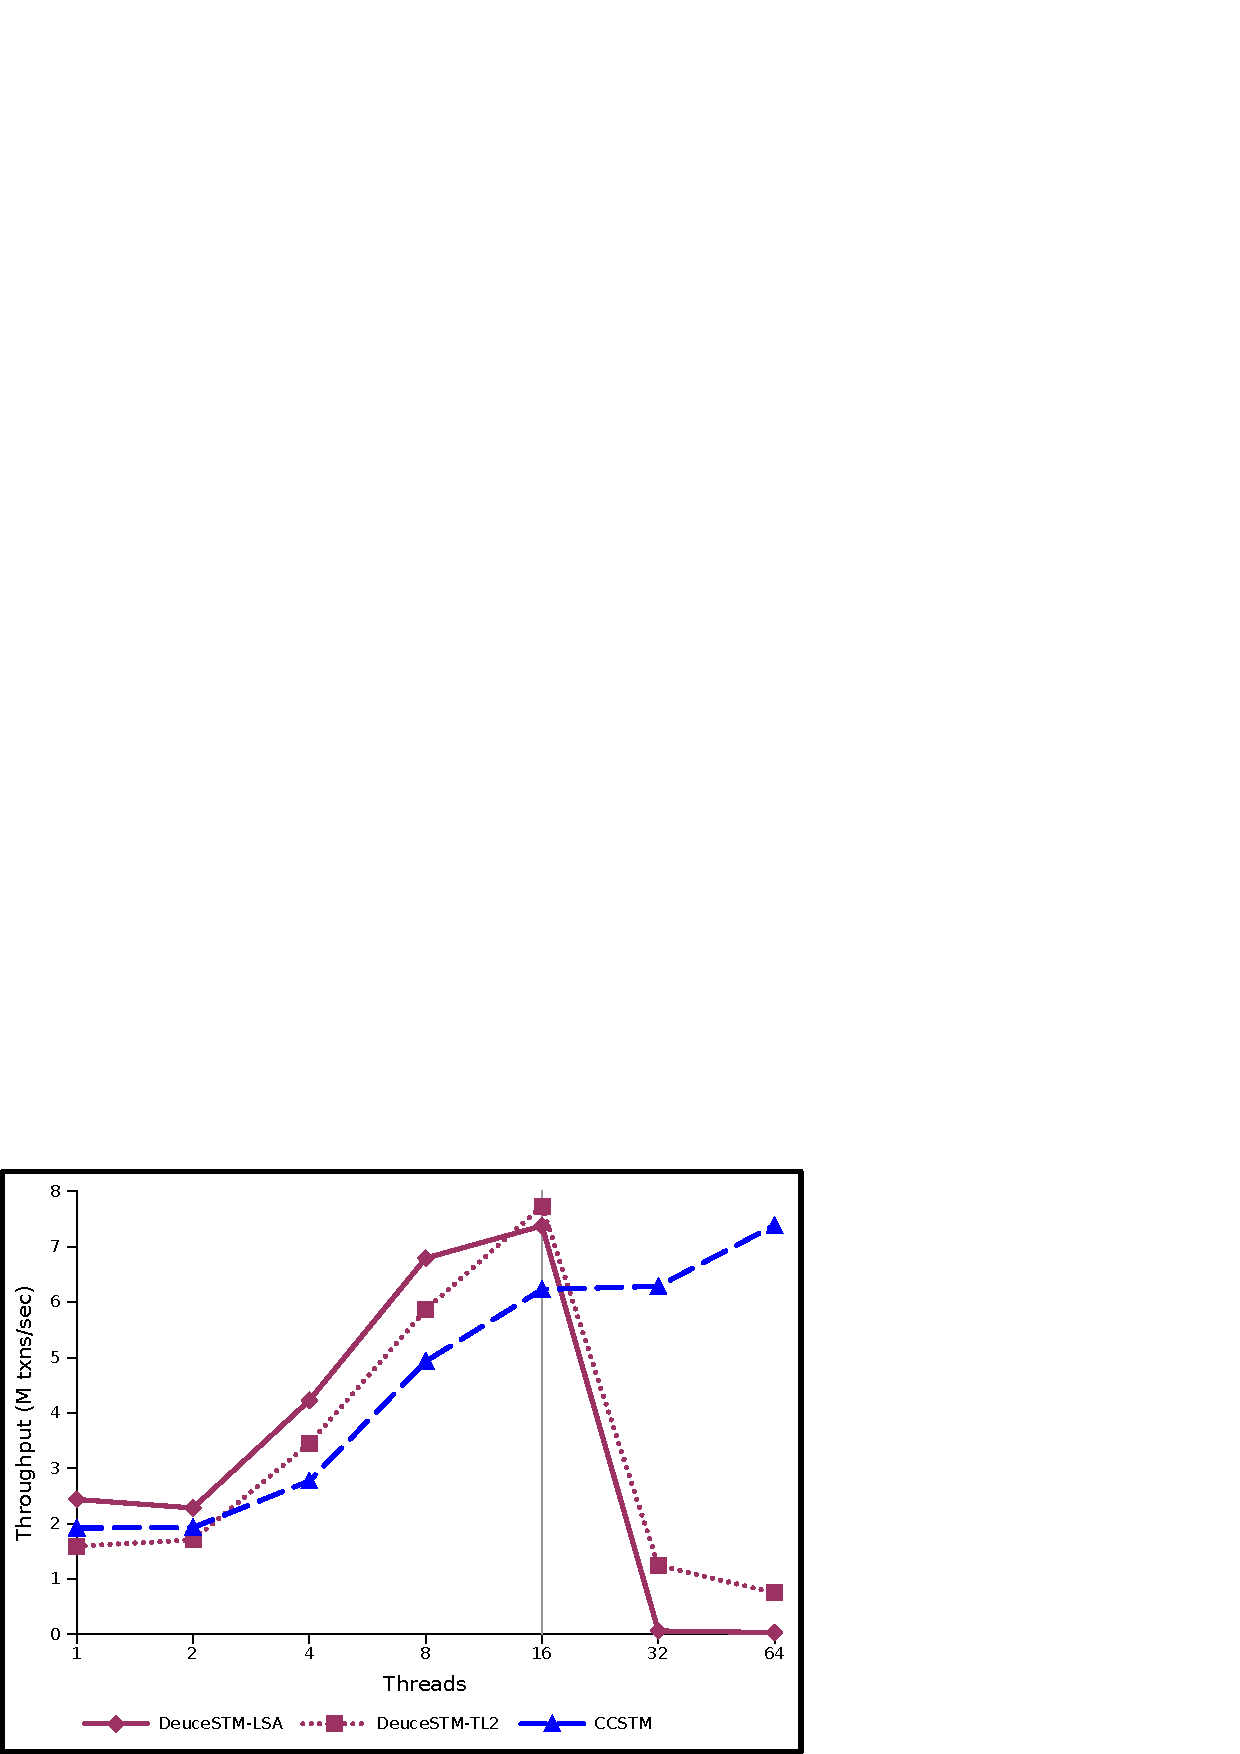
\includegraphics[clip=true,width=3in]{build/low_cont}

\caption{Throughput for the bank benchmark in a low contention scenario,
on a machine with 16 hardware thread contexts.  The number of accounts
is 64 times the number of threads.}

  \label{fig:lowcont}
\end{figure}

\begin{figure}
  \centering 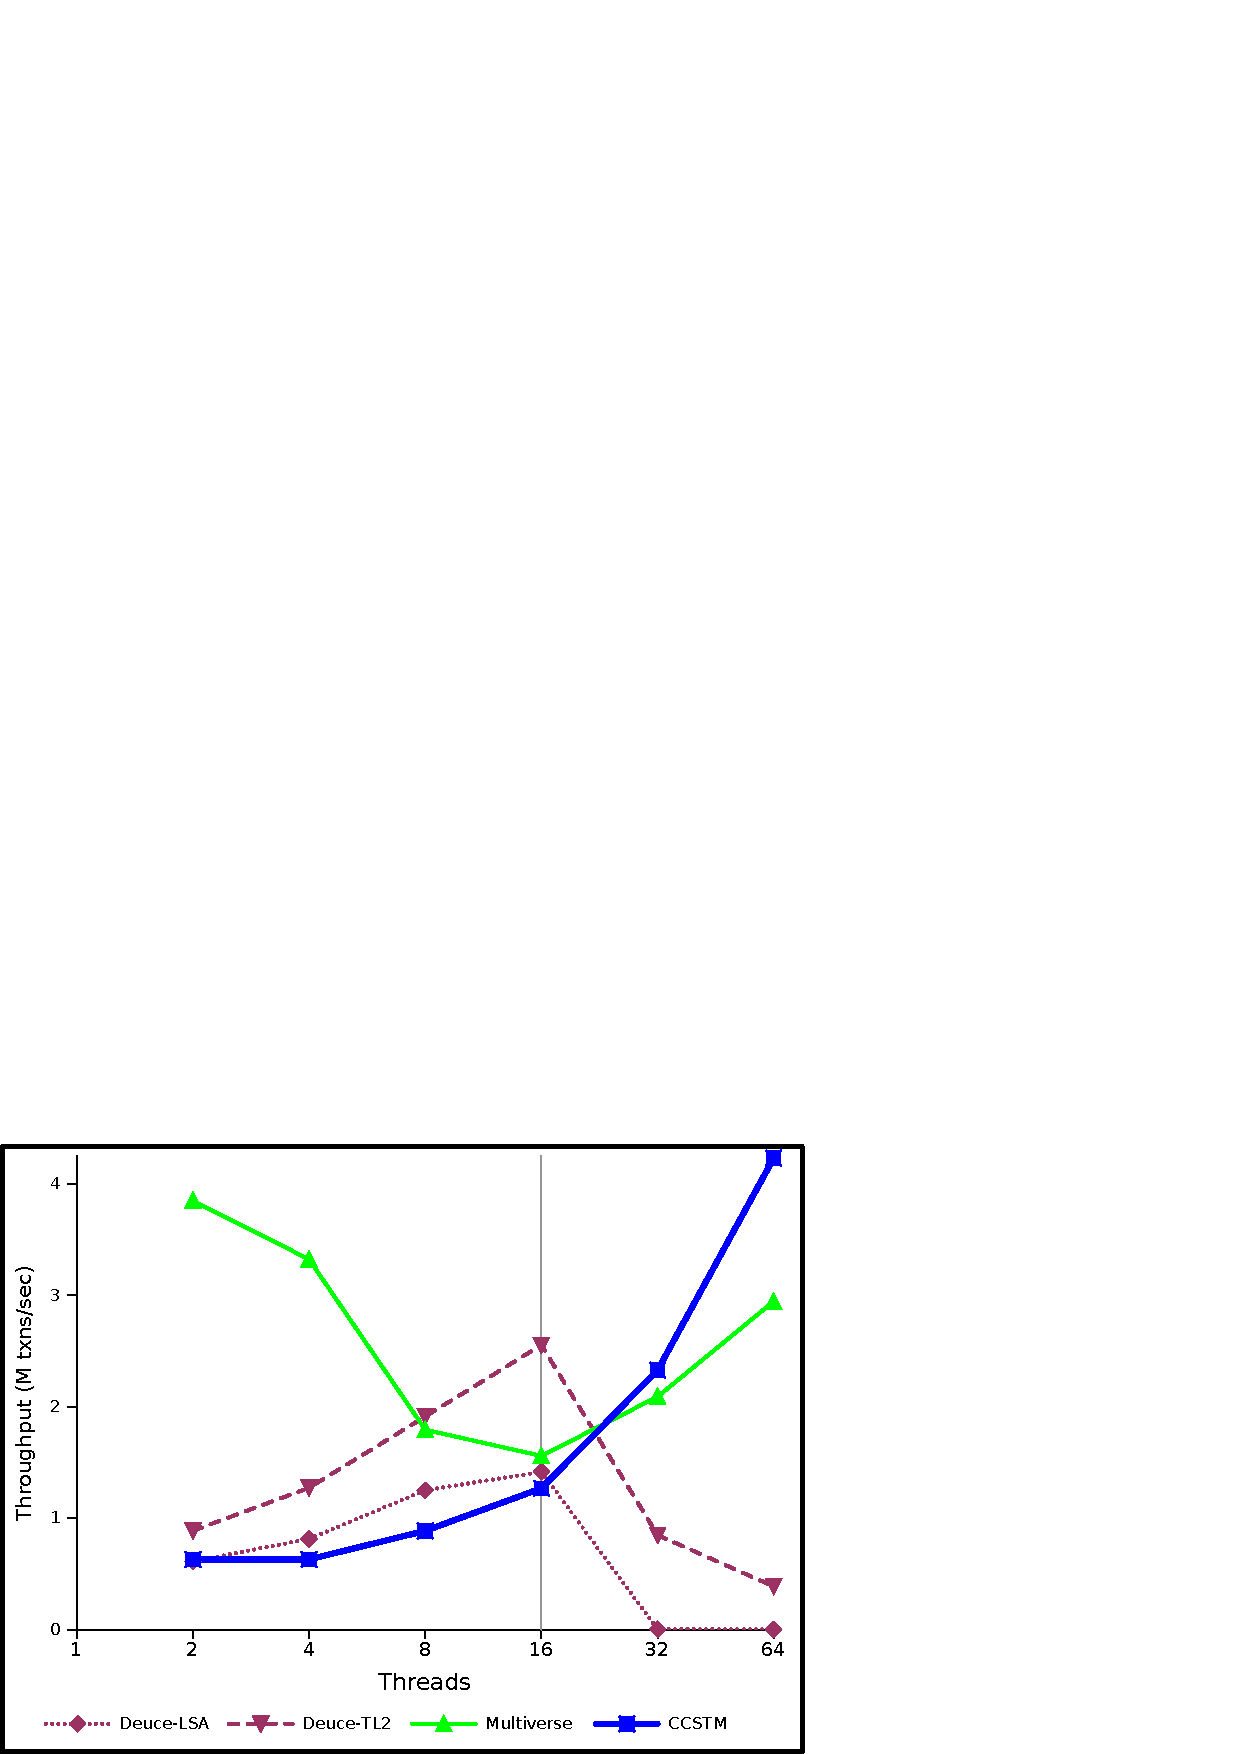
\includegraphics[clip=true,width=3in]{build/high_cont}

\caption{Throughput for a high contention scenario.  The number of accounts is
equal to the number of threads.  Each transaction touches two accounts.}

  \label{fig:highcont}
\end{figure}

To verify that CCSTM's library-based design does not impose a prohibitive
performance penalty, we compared it to Deuce STM, an STM for the JVM that
performs bytecode rewriting during class loading~\cite{deucestm}.

Experiments were run on a Dell Precision T7500n with two quad-core
2.66Ghz Intel Xeon X5550 processors, and 24GB of RAM.  Hyper-Threading was
enabled, yielding a total of 16 hardware thread contexts.  We used Scala
version 2.7.7.  We ran our experiments in
Sun's Java~SE Runtime Environment, build 1.6.0\_16-b01, using the HotSpot
64-Bit Server VM.  Deuce STM was version 1.2.0.
%We enabled dynamic escape analysis and compressed
%oops.

We performed a direct encoding of Deuce STM's bank benchmark into
Scala+CCSTM, and compared this version to the Java original running under
both the TL2 and LSA variants of Deuce STM.  (We were not able to use
Deuce STM to execute Scala code transactionally, due to a verifier error
in the instrumented classes.)  This benchmark includes its own harness,
which we configured so that no overdrafts were triggered.  We used a
4 second warmup, and then measured the number of transactions committed
during 10 seconds, averaging across three invocations of the JVM.  For the
low-contention experiment (Figure~\ref{fig:lowcont}) we set the number
of accounts to 64 times the number of threads.  For the high-contention
experiment (Figure~\ref{fig:highcont}) we set the number of accounts to
the number of threads.  Single-threaded execution is not included in the
high-contention setup, as it has no contention.  Because at most
16 threads are executing at any time, the high-contention runs have
fewer conflicts at 32 and 64 threads than for lower thread counts.

The TL2 version of Deuce STM is faster than CCSTM for both experiments when
the multi-threading level is less than or equal to one.  The difference
is largest for the high-contention scenario, where threads are often
obstructed.  Deuce STM does not block threads that cannot proceed, and it
does not even use sleeps or yields.  This strategy works well when every
thread gets its own hardware context, but results in a catastrophic
performance dropoff for higher thread counts.  CCSTM's synchronization
implementation is more expensive, but yields stable performance even at
high multi-threading levels.

Deuce STM and CCSTM have different algorithms and engineering tradeoffs,
so these experiments do not allow us to exactly measure the overhead
imposed by the library-only design.  They do demonstrate, however,
that any overhead that does exist is small enough to be tolerable.
